\section{Abstractions for NDA}
\label{sec:abstractions}

\begin{quote}
{\em Synthesis implies a bridge between two layers of abstraction} -- A. Sangiovanni-Vincentelli~\cite{alberto}
\vspace{-2mm}
\end{quote}

\begin{figure}[t]
\centerline{
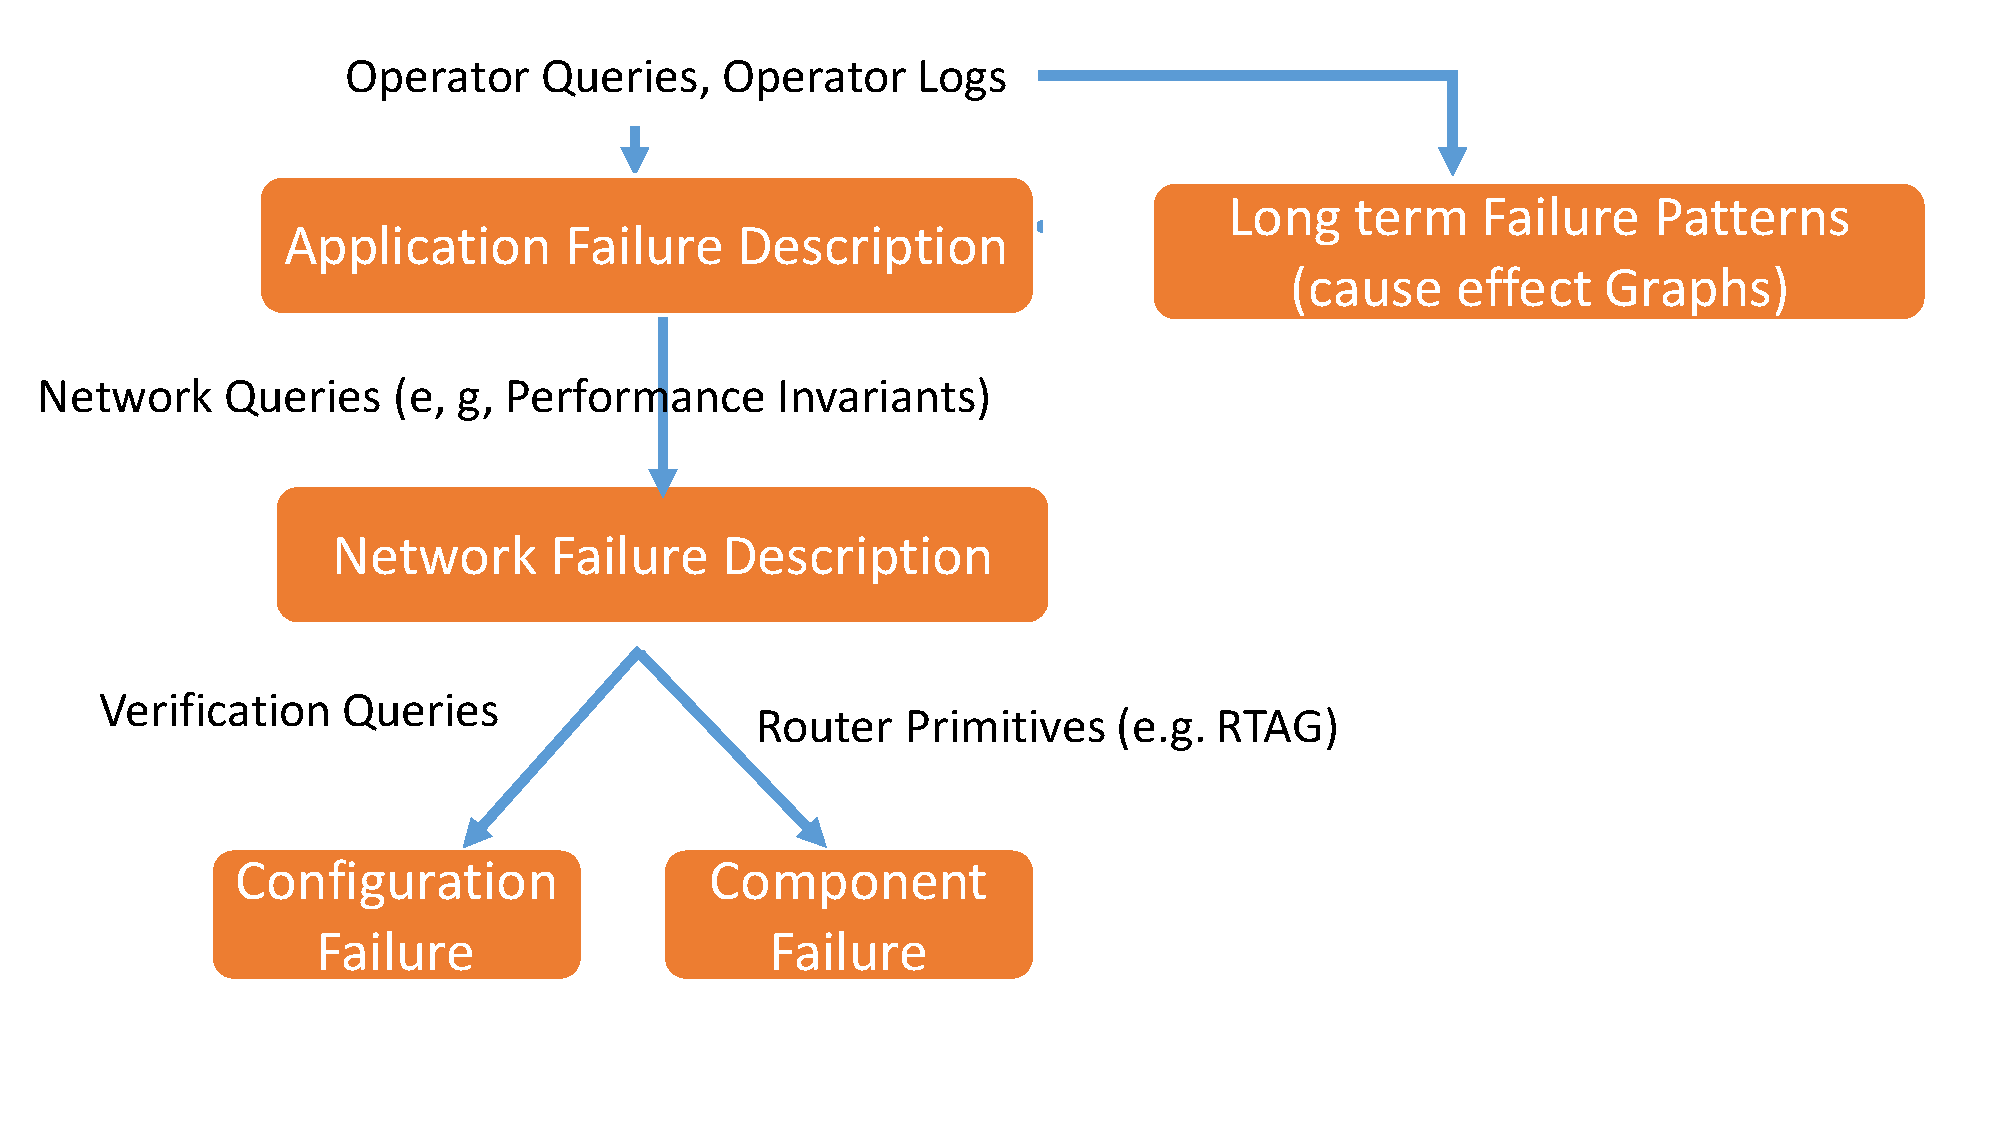
\epsfig{file=NDA-abstractions-new.pdf, height=4in}
}
\caption{\label{fig:abstractions} The layers of abstraction in NDA.}
\vspace{-5mm}
\end{figure}

Abstractions were key to the success of EDA~\cite{malik}. By steadily
raising the level of abstraction for designers, EDA allowed complex
chip designs to be developed using high-level behavioral models that
are mapped to blocks, to logic gates, and finally to lists of
wires. Although early efforts in EDA focused on bottom-up
verification, later innovation allowed synthesis between abstraction
levels.

\paragraph*{Abstractions for NDA}
%
Our proposal seeks to develop an analogous but preliminary set of \emph{interconnected} abstractions for NDA. Networks already have
abstractions for packet delivery (TCP and IP~\cite{kurose}) and for
packet forwarding (SDN-inspired flow
rules~\cite{Ethane,4DControlPlane,shenker-abstractions}) but do not have abstractions for
designing and configuring the network itself (or components
thereof). To that end, we have identified an initial set of layers of
a network that will frame our proposed research
(Figure~\ref{fig:abstractions}): {\em network diagnosis}, {\em router hardware}, (not a focus of this grant),  {\em packet schedules}, {\em routes}, and {\em topology}.


We aim to define abstractions at each of these layers of a network,
which can then be leveraged both for synthesis (from a higher to a
lower layer) and verification (from a lower to a higher layer).
Relative to EDA, these tasks are complicated by the fact that (a)
networks exhibit fine-timescale dynamics and evolve over long
timescales and (b) network design will need to incorporate human input
in the design process. As such, synthesis and verification for NDA is
a \emph{continuous} activity over the entire network lifecycle.  We
overview the goals of each proposed abstraction in the following
paragraphs; Section~\ref{sec:approaches} describes our proposed work
in detail and sets it in the context of related work.

% In the following paragraphs, we discuss our
% research in synthesis and verification, achieved through pairwise
% inter-disciplinary collaborations.

\paragraph*{NDA Research: Mapping Between Abstractions}
%

At the highest level, we assume that a network is meant to run networked
applications with application level service level requirements often expressed
by SLAs, ranging from loose (e.g., email, FTP, precision agriculture) to medium (video conferencing, VoIP, connected cards), to stringent (visualization, 
telesurgery) in terms of banswidth, latency, and jitter.

The first level abstraction (see topmost layer in Figure~\ref{fig:abstractions}) then is a {\em network topology} to run the applications}.  In our vision, each
abstraction layer corresponds to a tool.  For example, we envision a topology tool wherein an architect specifies traffic growth forecasts, resiliency requirements and components like routers and links, and the tool produces the physical network.  Many cloud providers including Google~\cite{condor} and Microsoft already have such tools but these are proprietary and would not apply to a rural network like Air Jaldi.  

Imagine an open source tool that can design a physical network whether
for a rural network that uses VoIP (1000 users in 12 villages, using wireless links and FPGA based routers) or a larger data center network for Google (10, 000 users for Google Applications using high end Cisco routers).    The Condor system at
Google~\cite{condor} recently proposed a delarative Topology
Description Language (TDL) to specify abstract topology connectivity
and uses a constraint solver to generate topologies {\bf S4} but it only automates
some limited aspects of topology design.


Once the physical
network is laid out, the baton passes from the network architect to the network
operator. Applications must specify their traffic demands and performance objectives. Merlin allows an operator to specify a policy to set up routes and packet schedules.  Note that unlike conventional networks, these routes and schedules can be  tuned to application objectives.  Thus the first job is to layout application traffic on specific network paths subject to policy restrictions and to optimize enterprise objectives.  For example, email and Voice Over IP could be ``laid out'' over the physical network where VoIP is sent on multiple paths while email is sent on only one path.
Thus we envisage a routing tool that maps from application objectives and a 
physical network design to routes for each application traffic.  


The next abstraction is {\em packet schedules}.   While packet schedules are
today largely decided by each router in decoupled fashion, work such as 
Fastpass~\cite{fastpass} argues that even packet schedules could be computed by
a tool and passed to each router.  For example, the schedule could decide that
in some routers, Voice Over IP gets priority scheduling over email. when the two traffic classes intersect at that router.

Of course, when churn occurs such as DoS or monsoon in a rural network or a fiber cut in a data center, the route are reconfigured automatically based on operator specification (ecommerce takes priority over web surfing during monsoon for rural
networks, customer traffic gets priority over analytics in a data center.  Another important kind of churn is the specification of new application requirements by the operator.  For example, in a rural network if the operator adds a new tele-surgery application this can change the layout of the other packets and the schedules at 
each router.

While our example uses rural networks, the same idea applies to say Pfizer doing visualization of genome data and Augmented Reality for drug design, or Google adding connected cars, or John Deere adding precision agriculture.

These abstractions (topology, routes, schedule) compile down to a back end
that can be a source routed network with FPGA based routers (for rural 
networks), a  conventional network with Cisco routers with BGP and scheduling parameters set by the higher abstraction levels, or even a P4 router based on say the Broadcom chip and routes set up by an OpenFlow controller.  This is the
next layer below that we call hardware.

In this layer, a router
designer combines hardware {\em tiles} such as multiplexers and
memories to make hardware blocks that comprise a pipeline {\em stage}.
Designing router pipelines is a field that is greatly in need of tools and
the ability for reseachers to build tools (as opposed to proprietary tools used
at Cisco and Google) has had an inflection point since the advent of the
P4 language~\cite{P42016}.  

For focus, this grant will {\bf not focus on router design tools}.  We will however,
investigate debiugging primitives in router hardware) the bottom most layer 
especially as it relates to network debugging, the bottom most layer.


Various synthesis and verification tasks operate on the
router and scheduling abstractions. One is the synthesis of router-level
topology of an entire network from constraints on traffic and
connectivity~\cite{condor}. A related synthesis task requires the
network architect to adapt to traffic changes via {\em traffic
  engineering} that maps measured {\em traffic matrices} over some
duration to route configuration commands at routers.  Abstractions
also enable synthesis and verification between high-level network
\emph{policies} and their low-level configurations.

A network operator also needs to
monitor and debug the network.  Ideally, the operator should issue
{\em network performance queries} at an autonomous system level (e.g.,
compute traffic matrix) and have these mapped to performance commands
at each router (e.g., read byte counter).  On a longer time scale, the
network architect needs to extract, from logs of network faults
captured (often annotated by a network operator), a higher-level
{\em failure model}, which can be used to target efforts to improve
reliability. We lump all these concerns into the bottommost level

Notice that our tools work on designing specialized networks within a single
Autonomous Systems or AS where the architect and operator can control the 
entire network.  Examples include rural networks, data center networks ad 
enterprise networks. Of course, individual networks are interconnected to form the Internet .  We do not focus on such Network Design Automation ``in the large''
because we feel that is precisely the specialized context (rural networks, 
data center networks) that can allow novel language based synthesis and
verification tools to work.

\paragraph*{Our Approach:} While there exist point solutions at some of
these layers for certain tasks, these abstractions are neither {\em
  complete} or {\em interconnected}. We will produce a complete and
interconnected set of abstractions from topology down to schedules.
Interconnecting abstractions allows us to build
an end-to-end system from routers to rural networks, as we propose
in our evaluation.



 
